\documentclass{beamer}

\usepackage[utf8]{inputenc}
\usepackage{default}
\usepackage{graphicx}
\usepackage{bbding}


% TODO Learn what this does
% source
% http://tex.stackexchange.com/questions/15952/layout-of-multiple-lines-footnotes
% this is a way to adjust foot note so it can be cutted into multiple lines
\makeatletter
\renewcommand\@makefntext[1]{\tiny\rightskip=25em\hskip0em\@makefnmark#1}
\makeatother

\makeatletter
\newcommand*{\rom}[1]{\expandafter\@slowromancap\romannumeral #1@}
\makeatother


% shows how to change default (blue) colours in the default beamer theme
% found here: http://joerglenhard.wordpress.com/tag/latex/
\definecolor{WaterlooRed}{RGB}{145,11,46}
\setbeamercolor{title}{fg=WaterlooRed}
\setbeamercolor{frametitle}{fg=WaterlooRed}
\setbeamercolor{structure}{fg=WaterlooRed}

% adds logo in the footer
\logo{
\includegraphics[scale=.25]{img/csuow}}

\title[]{MicroFuge: A Middleware Approach to Providing Performance Isolation in Cloud Storage Systems}
\author[Akshay Singh, Xu Cui, Benjamin Cassell, Bernard Wong and Khuzaima Daudjee]{Akshay Singh, Xu Cui, Benjamin Cassell, Bernard Wong and Khuzaima Daudjee}
\institute{
\includegraphics[scale=0.25]{img/UniversityOfWaterloo_logo_vert_rgb.png}}
\date{{\tiny\today}}

\begin{document}

\begin{frame}
  \titlepage
\end{frame}


\begin{frame}
  \frametitle{Cloud Computing}
  \begin{itemize}
  \item Cloud computing leverages economies of scale to improve resource sharing.
  \item This comes at the costs of reduce isolation between tenants.
  \end{itemize}
    \centering
    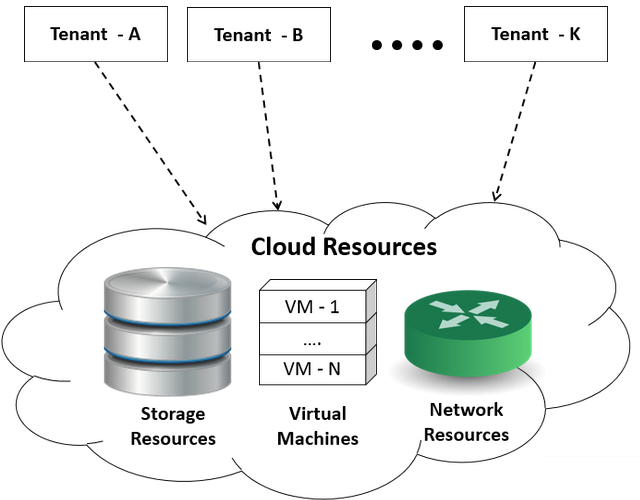
\includegraphics[scale=0.26]{img/icdcs1.png}

\end{frame}


\begin{frame}
  \frametitle{Resource Allocation in Cloud Datacenters}
  \begin{itemize}
  \item CPU - Virtualization Technologies
  \item Memory - Virtualization Technologies
  \item Network - Software Defined Networks
  \item Storage
    \begin{itemize}
    \item Virtualization Technologies degrade overall performance of the deivce.
    \item Cloud providers offer shared, distributed storage services.
    \item Multiple tenants: \textcolor{red}{Performance Interference}
    \end{itemize}
  \end{itemize}
\end{frame}

\begin{frame}
  \frametitle{Typical Use Cases}
  \begin{itemize}
  \item A lot of services are backed up by cloud storages services today.
  \item Response time matters. A longer loading time can drive your customers away.
    %% \centering
    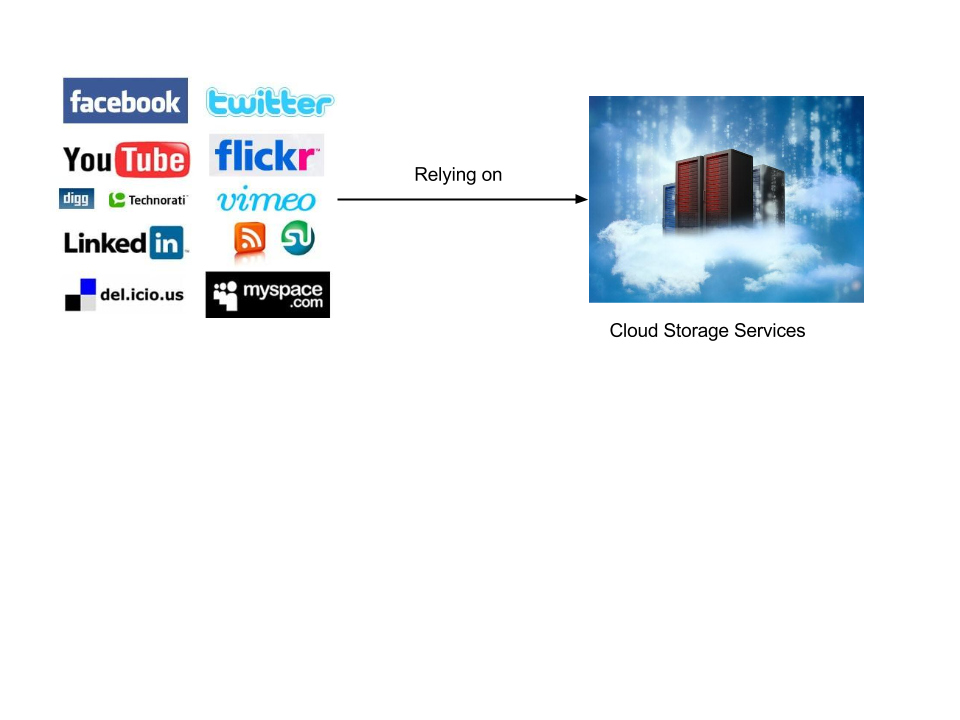
\includegraphics[scale=0.26]{img/A_Cloud_Example.png}
  \end{itemize}
\end{frame}


\begin{frame}
  \frametitle{Agenda}
  \begin{itemize}
  \item[\Checkmark] Background and Motivation
  \item MicroFuge
    \begin{itemize}
    \item Deadline Cache
    \item Deadline Scheduler
    \end{itemize}
  \item Evaluation
  \item Conclusion
  \end{itemize}
\end{frame}

\begin{frame}
  \frametitle{MicroFuge}
  \begin{itemize}
    \item A new distributed caching and scheduling middleware that provides performance isolation.
      \begin{itemize}
      \item Middleware - Reduce the barrior to adoption.
      \item Distributed - Seamlessly scalable.
      \item Multiple layers - Can be selectively adopted.
      \item Performance isolation - Relying on an emperically-driven
        performance model of the underlying storage system.
      %% model the isolation with deadlines?
      \end{itemize}
  \end{itemize}
\end {frame}


\begin{frame}
  \frametitle{Major Contributions of MicroFuge}
  \begin{itemize}
    \item \textbf{Deadline Cache (DLC)} - Deadline-aware, model-driven distributed
      caching system.
    \item \textbf{Deadline Scheduler (DLS)} - Deadline-aware distributed scheduling system.
    \item \textbf{Evaluation} - Demonstrates the effectiveness of MicroFuge in
      an EC2 deployment using the YCSB benchmark.
  \end{itemize}
\end {frame}



\begin{frame}
  \frametitle{MicroFuge at a Glance}
  \begin{itemize}
    \item MicroFuge \textit{read} operation interface.
    %% \centering
  \end{itemize}
    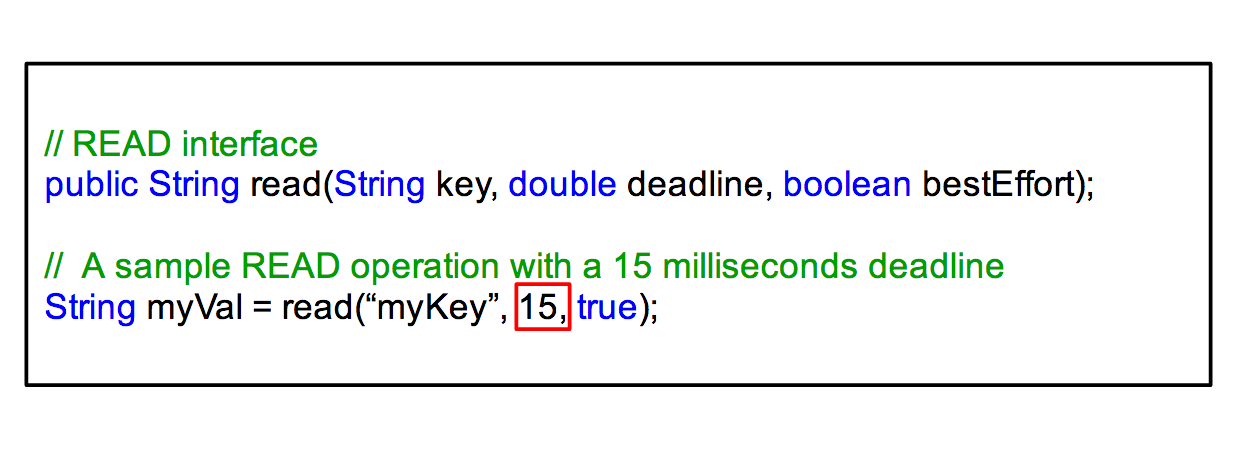
\includegraphics[scale=0.40]{img/MicroFuge_protocol.png}

\end{frame}


\begin{frame}
  \frametitle{Full MicroFuge - An example}
  \begin{itemize}
    \item Sample timeline for a read request from a client. For this request,
      the requested item is not in contained in the cache.
  \end{itemize}

  \begin{figure}
    \begin{center}
      \centerline{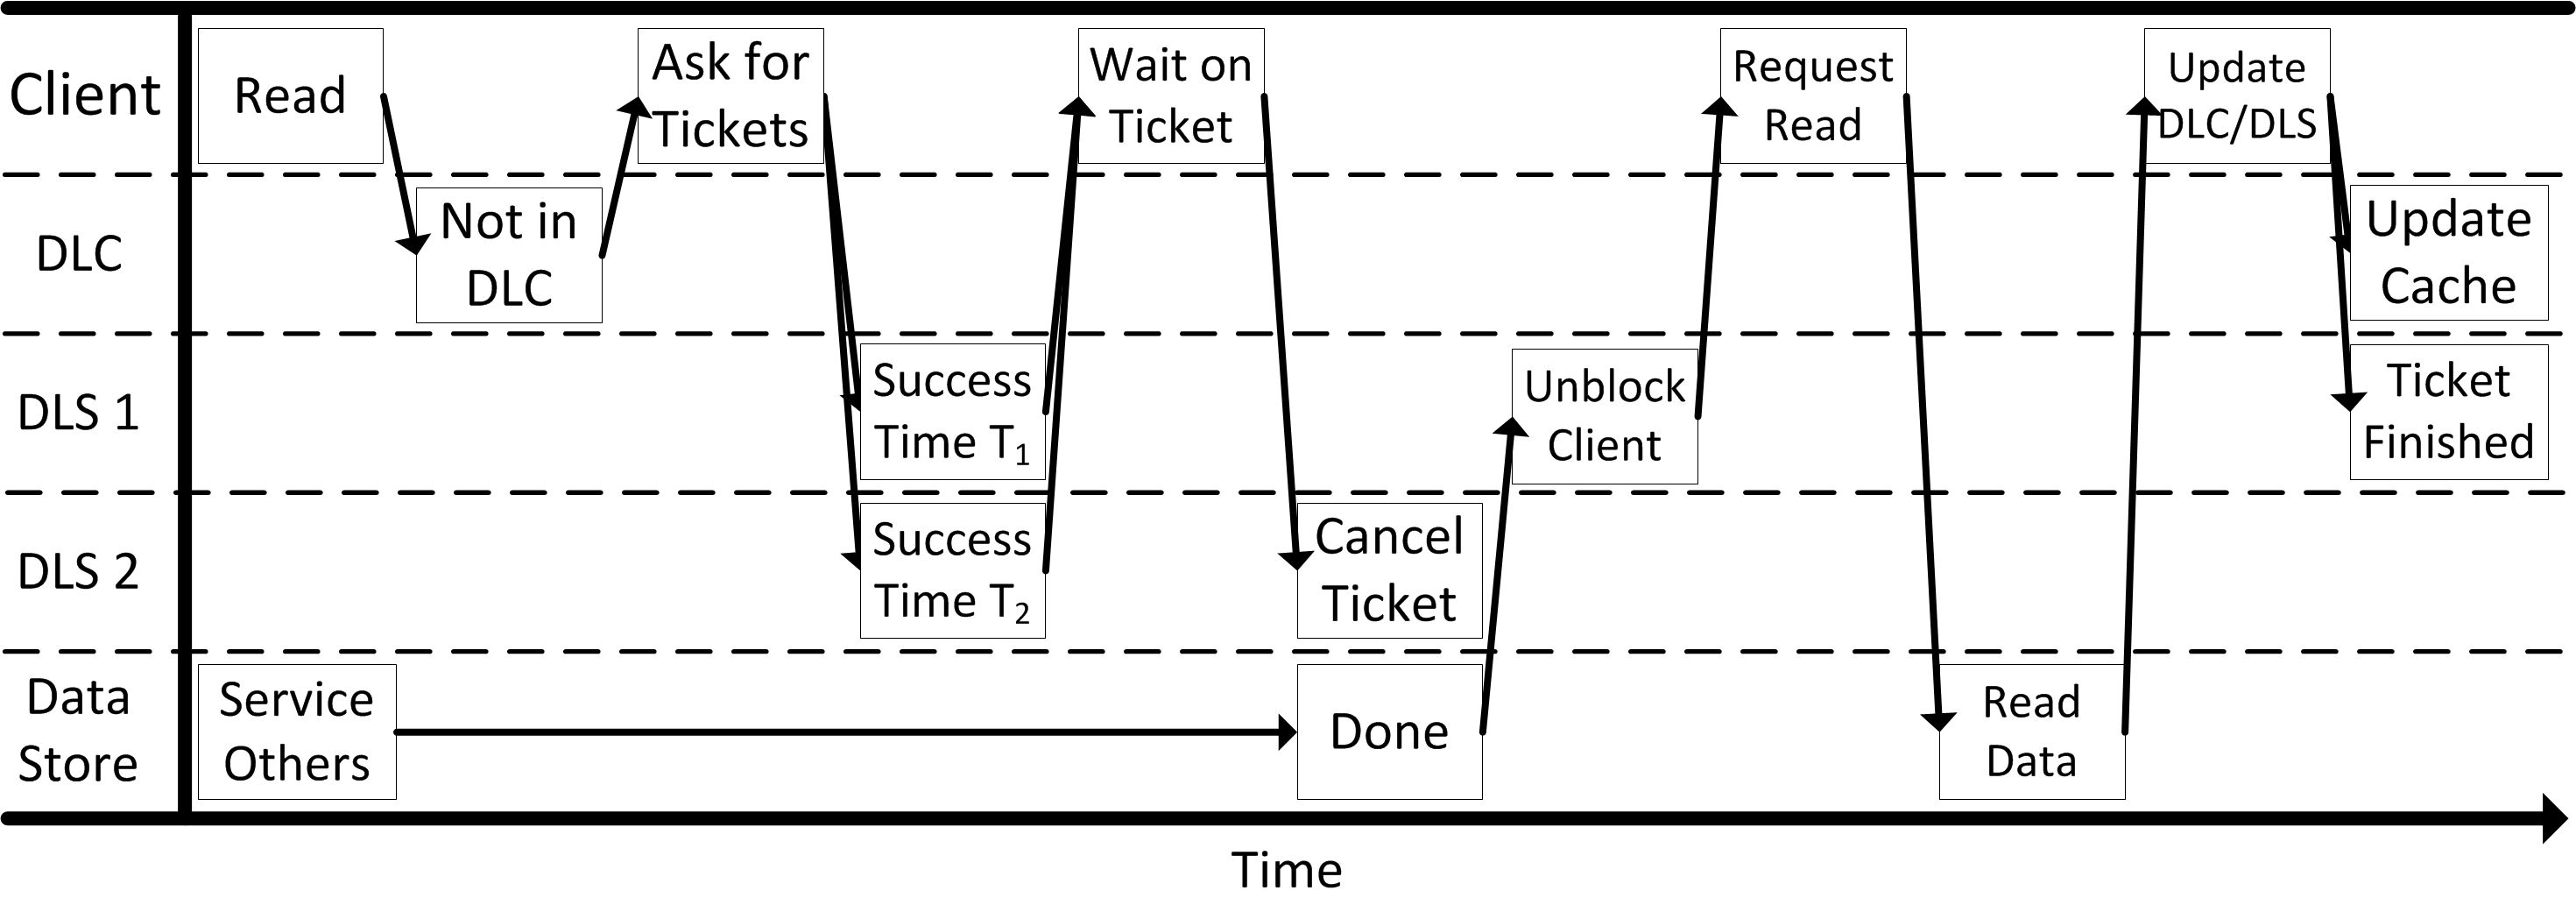
\includegraphics[scale=0.60]{img/RequestTimelineHorizontal.png}}
    \end{center}
  \end{figure}
\end {frame}

\begin{frame}
  \frametitle{Agenda}
  \begin{itemize}
  \item[\Checkmark] Background and Motivation
  \item[\Checkmark] MicroFuge
    \begin{itemize}
    \item Deadline Cache
    \item Deadline Scheduler
    \end{itemize}
  \item Evaluation
  \item Conclusion
  \end{itemize}
\end{frame}


\begin{frame}
  \frametitle{Deadline Cache (DLC) - Architecture}
  \begin{itemize}
  \item Major components - Multiple LRU queues for deadline-aware eviction and
    a performance modeling component.
  \end{itemize}
  \begin{figure}
    \begin{center}
      \centerline{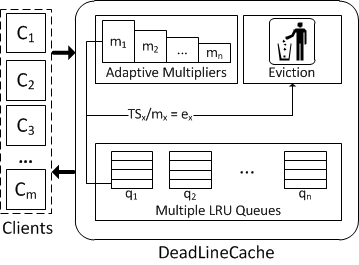
\includegraphics[scale=0.8]{img/DLC_arch.png}}
    \end{center}
  \end{figure}
\end{frame}


\begin{frame}
  \frametitle{DLC - Adaptive Caching}
  \begin{itemize}
  \item Multiple queues - Maintain the ordering of key-value pairs spanning
    different deadline ranges.
  \item Queue specific multiplier - Adaptively computed to model the likelihood
    of deadline misses within a deadline range.
  \item Modified Recency Value (MRV) - apply the multiplier to the time elapsed
    since the last access to an item.
  \item Eviction - Item with largest MRV is evicted.
  \end{itemize}
\end{frame}


\begin{frame}
  \frametitle{DLC Interface Functions}
  \begin{itemize}
    \item Sample \textit{get, put} interface to manipulate the deadline-aware cache.
  \end{itemize}
  \begin{figure}
    \begin{center}
      \centerline{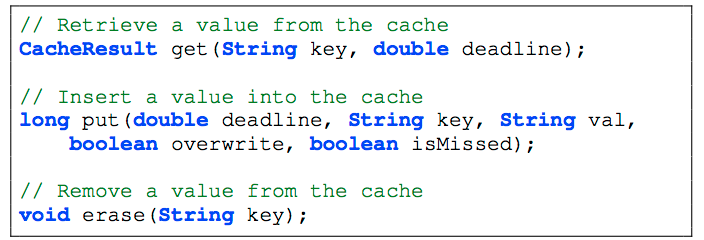
\includegraphics[scale=0.45]{img/DLC_interface.png}}
    \end{center}
  \end{figure}
\end{frame}

\begin{frame}
  \frametitle{DLC - Advantages}
  \begin{itemize}
  \item Adaptivness
  \item Efficient Computation
  \item Deadline Aware
  \item Tunable
  \end{itemize}
\end{frame}

\begin{frame}
  \frametitle{Agenda}
  \begin{itemize}
  \item[\Checkmark] Background and Motivation
  \item MicroFuge
    \begin{itemize}
    \item[\Checkmark] Deadline Cache
    \item Deadline Scheduler
    \end{itemize}
  \item Evaluation
  \item Conclusion
  \end{itemize}
\end{frame}

\begin{frame}
  \frametitle{Deadline Scheduler (DLS) High-level Architecture}
  \begin{itemize}
    \item
  \end{itemize}
  \begin{figure}
    \begin{center}
      \centerline{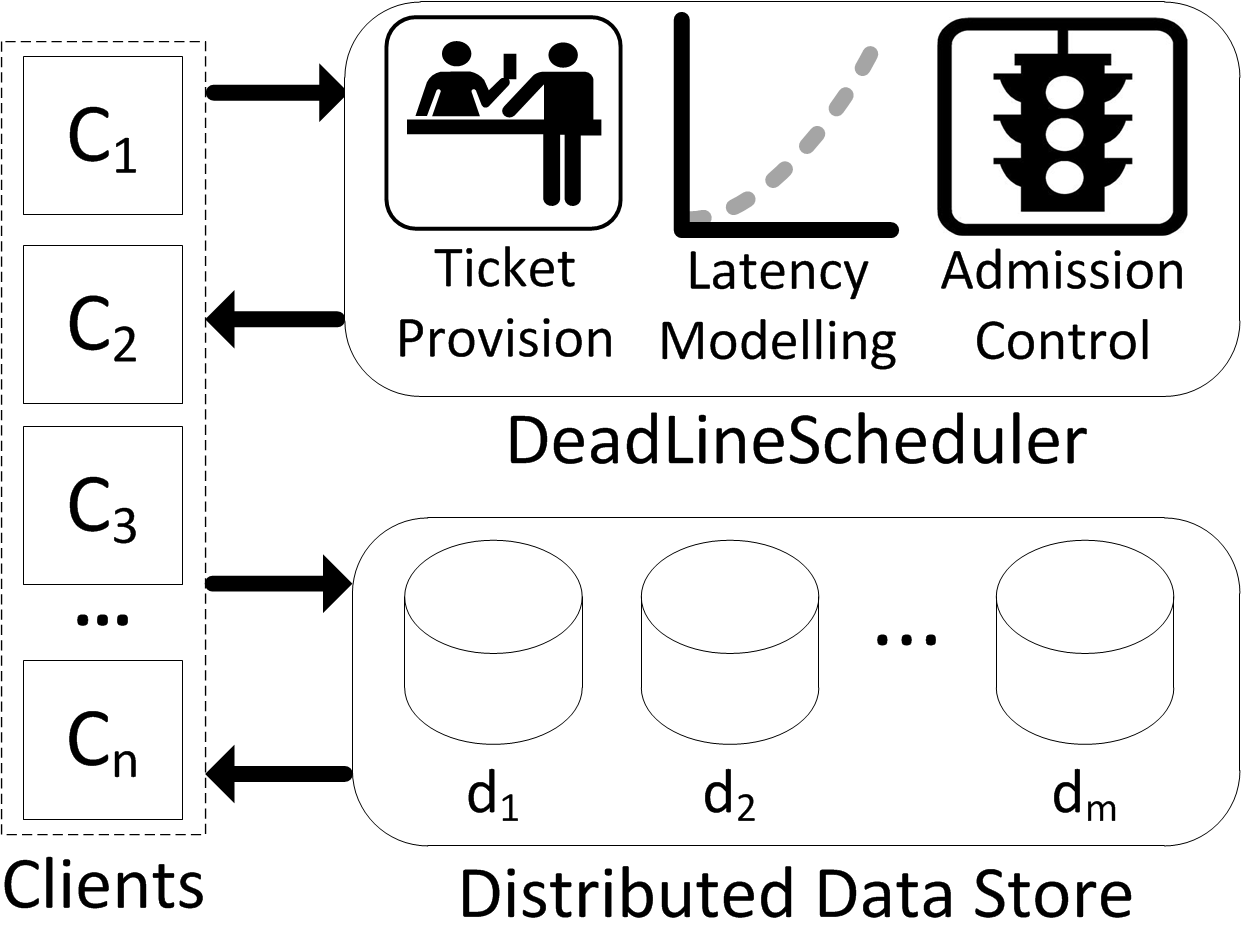
\includegraphics[scale=0.90]{img/DLS.png}}
    \end{center}
  \end{figure}
\end{frame}


\begin{frame}
  \frametitle{Agenda}
  \begin{itemize}
  \item[\Checkmark] Background and Motivation
  \item[\Checkmark] MicroFuge
    \begin{itemize}
    \item[\Checkmark] Deadline Cache
    \item[\Checkmark] Deadline Scheduler
    \end{itemize}
  \item Evaluation
  \item Conclusion
  \end{itemize}
\end{frame}


\begin{frame}
  \frametitle{Experimental Setup - The Cluster}
  \begin{itemize}
    \item Twenty-node test cluster on AWS. Each cluster node is an m1.medium
      EC2 instance.
  \end{itemize}
\end{frame}


\begin{frame}
  \frametitle{Agenda}
  \begin{itemize}
  \item[\Checkmark] Background and Motivation
  \item[\Checkmark] MicroFuge
    \begin{itemize}
    \item[\Checkmark] Deadline Cache
    \item[\Checkmark] Deadline Scheduler
    \end{itemize}
  \item[\Checkmark] Evaluation
  \item Conclusion
  \end{itemize}
\end{frame}


\begin{frame}
  \frametitle{Conclusion}
  \begin{itemize}
    \item Predictable performance is necessary in multi-tenant environments.
    \item MicroFuge - A middleware approach to performance isolation in cloud
      storage sytems.
    \item Deadeline awareness - Reduces deadline miss rate from over 20\% to
      less than 5\%.
  \end{itemize}
\end{frame}

\end{document}
